\part{Intro}
\label{pa:intro}
\chapter{Introduction}
\section{Oversight}
\begin{figure}
    \lable{fig:testfig}
    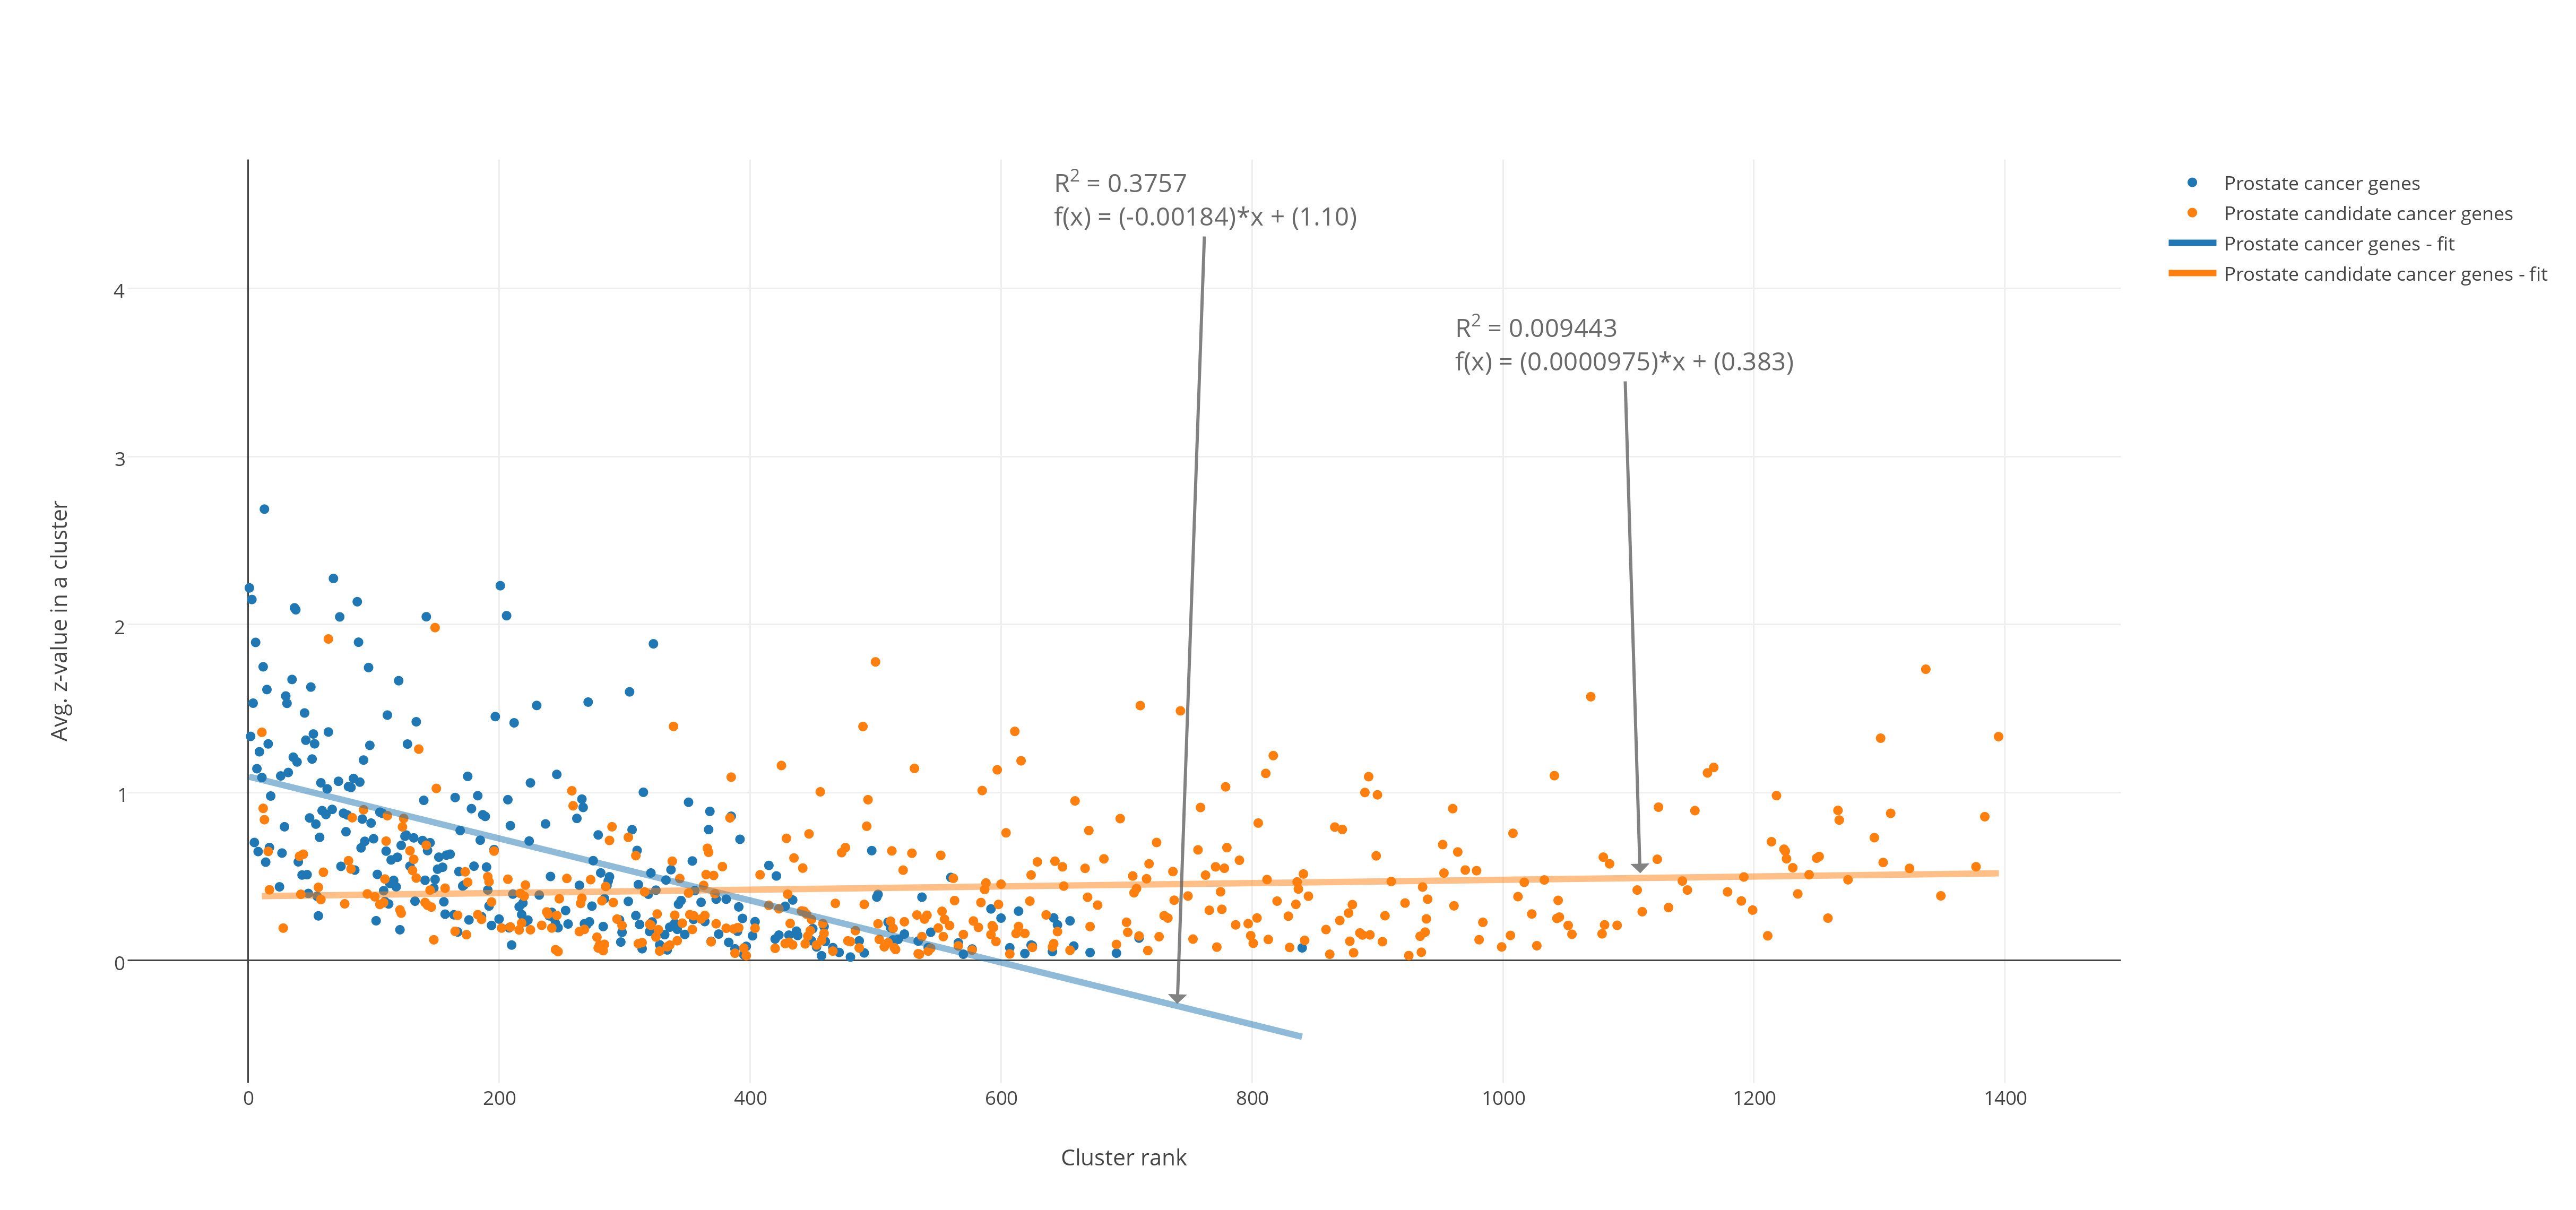
\includegraphics{newplot}
    \caption{trololol}
\end{figure}
%% TODO: fix this shit!
To this day we still struggle with cancer. Even with all our modern equipment
and knowledge we have still not been able to tame this horrible disease. This
thesis is about implementing and using a tool named Ranklust. It is not a
standalone tool, but rather a contribution to a Cytoscape plugin named
clusterMaker2\cite{cm2}\cite{cm2-github}. The goal of this tool is to rank
clusters created from Protein-Protein Interaction (PPI) networks in Cytoscape.
The ranks will be based on different node and edge attributes in the network.
The resulting ranks will also indicate which clusters can be seen as cluster
biomarkers, and which genes could be considered to be single gene candidate
biomarkers. 

\chapter{Background}
\section{Biomarkers}
A biomarker is a "biological measure of a biological state"
\cite{biomarker1}. Among other things, it can be represented by the levels of
a specific protein in our blood, a specific gene, or a combination the two.
Biomarkers can be used for different purposes. They can be used to measure the
effect of cancer drug treatment. That the drug does what it is supposed to do.
It can be used to predict disease development or the current stage of the
disease. Here is a list of what biomarkers currently are being used for:
\\\\
\textbf{Usages for biomarkers:} \cite{beyondpsa}
\begin{itemize}
    \item Disease disposition
        \begin{itemize}
            \item What is a patient's risk of developing cancer in the future?
        \end{itemize}
    \item Screening
        \begin{itemize}
            \item Does earlier detection of patients with cancer decrease
                mortality?
        \end{itemize}
    \item Diagnostic
        \begin{itemize}
            \item Who has cancer? What is the grade of the cancer?
        \end{itemize}
    \item Prognostic
        \begin{itemize}
            \item What clinical outcome is most likely if therapy is not
                administered?
        \end{itemize}
    \item Predictive
        \begin{itemize}
            \item Which therapy is most appropriate?
        \end{itemize}
    \item Monitoring
        \begin{itemize}
            \item Was therapy effective? Did the patient's disease recur?
        \end{itemize}
    \item Pharmacogenomic
        \begin{itemize}
            \item What is the risk for adverse reaction to the prescribed
                therapeutic dose?
        \end{itemize}
\end{itemize}
\textbf{Characteristics for a good biomarker:}
\begin{itemize}
    \item Safe and easy to measure
    \item Cost efficient to follow up
    \item Modifiable with treatment
    \item Consistent across gender and ethnic groups
\end{itemize}

%% New part in Motivation - should it stay or be rewritten?
The National Institutes of Health Biomarkers Definitions Working Group has
defined biomarkers as "a characteristic that is objectively measured and
evaluated as an indicator of normal biological processes, pathogenic process, or
pharmacologic responses to a therapeutic
intervention."\cite{biomarker2,biomarker3}. The World Health Organization (WHO)
has created a guideline for defining biomarkers: "almost any measurement
reflecting an interaction between a biological system and a potential hazard,
which may be chemical, physical or biological. The measured response may be
functional and physiological, biochemical at the cellular level, or a molecular
interaction". So a biomarker can be anything from the pulse of the heart or
blood pressure. In this thesis, I will see if we can get better and more
information from ranking gene clusters based on biomarker information. The
result could in the best case be a new biomarker in itself, and can be a step in
the direction of hierarchical biomarkers (biomarkers creating new biomarkers).

\subsection{Biomarkers and Clinical Endpoints} 
Some of the important characteristics of biomarkers is that they are objective
and quantifiable as biological processes\cite{biomarker3}. They are used as
a state indicator of the biological object that is under scrutiny. When the
biological object is a human being screened for cancer, biomarkers may help.

Biomarkers can be an indicator of how far cancer has progressed in the human
body, even though the human subject may feel no difference at all. It can also
be the opposite, that the human subject feels huge differences during several
weeks that the cancer might have developed at a grand scale, but the biomarkers
show no objective change. This proves that the human subject's experience and
sense of state that it is in does not necessarily have to correlate.

Clinical endpoints is the opposite\cite{biomarker3}. They describe how the
subjects feel or describe how they function. It is not as objective as
biomarkers and it demands more resources to gather the information, as the
subjects has to be interviewed in some form, rather than interpreting pure data.
But one thing has to be noted; patients does not seek treatment for cancer due
to their biomarkers being "off the charts". They seek treatment because they
feel that they do not feel ok or do not function sufficiently. So biomarkers are
not by any means far superior to clinical endpoints in all aspects.

Biomarkers can also be ruled out as a reliable predictor when population
differences are too big\cite{biomarker3}. As with clinical endpoints, people
describe their feelings differently and might hold information back. As pointed
out before, people's feelings are subjective, and different ways of interpreting
their own body's state might skew statistical results with erronous feedback.
Erronous feedback in this case can be examplified as two persons who are at the
exact same state of cancer, with the same prerequisites, but they report how
they feel differently. One person might be ignoring certain pains or lose hair
after radiation treatment, but not the other. This can be mitigated to some
degree with careful and accurate screening of patients admitted to treatment,
but a totally unified group in terms of how they describe pain and other
attributes that are interesting might be seen as borderline impossible. We are
after all humans and very much fallible.

\subsection{Prostate cancer statistics}
Statistics show that "In 2013, there were 1.4 million incident cases of prostate
cancer and 293 000 deaths"\cite{cancerburden2}. Taking population into
concideration together with the increasing incidence rates, we have had
a "3-fold increase in prostate cancer cases since 1990"\cite{cancerburden2}. 

\subsection{Specific biomarkers}
An example of a single molecule biomarker is the prostate specific antigen
(PSA). This is a protein produced by the prostate gland in male humans. The
identification of cancer with PSA is simple, the higher the level of PSA,
measured in ng/mL (nanograms per milliliter), the higher is the chance of the
patient having prostate cancer \cite{cancerfacts}.

Today PSA is used for both identifying and evaluating the current stage of
prostate cancer. This biomarker can be found by analyzing blood examples from
patients, thus fulfilling some of the demands for a good biomarker, but not all
of them. It is easy to measure and easy to acquire, but not reliable enough to
be used as the only marker to identify and determine the stage or remission of
prostate cancer. The low grade of reliability comes from the fact that even
though higher levels of PSA shows higher chance of having prostate cancer,
prostate cancer is not the only reason to have elevated levels of PSA
\cite{cancerfacts}. Namely inflammation and enlargement of the prostate. Though,
a man with both of these cases may or may not develop prostate cancer.

So the conclusion for the PSA biomarker is that it is not reliable enough and
are causing faulty treatment of prostate cancer that may not even exist. Because
even if a patient has prostate cancer, it may not be harmful, promoting the case
of not taking any action against it at all. So there is need for a new
biomarker, or at least a better way to diagnose and predict the right treatment.

\chapter{Big data in bioinformatics and networks as a tool in cancer research}
\section{Existing biomarkers}
The PSA biomarker is over 20 years old \cite{psa-age}. Through those years, it
has been discovered other and better biomarkers for prostate cancer than PSA.
Among those, PCA3, which is detectable through urine samples from patients. It
also has the benefit of not being affected by the size of the prostate gland
\cite{pca3-size}. But still the results could be better. Therefore, it has been
tried to combine these two biomarkers in order to see if it is beneficial to see
the results from each biomarker in light of each other \cite{beyondpsa}. The
results from these tests is that they complement each other to a level of
significance that makes it compelling to analyze them both to diagnose prostate
cancer. It is important to point out that even if these biomarkers are not the
best at indicating if a patient has cancer or not, these biomarkers are good at
indicating progression and recurrence of prostate cancer.

In the cases of pancreatic, lung, breast, brain and overian cancer, the somatic
distribution of single-nucleotide polymorphisms (SNP) has a few altered genes
that occur with a frequency higher than 10\%, and many other genes that are
mutated occur with a frequency of 5\% or lower\cite{pathway-network}. On the
other hand, prostate cancer has relatively few SNPs and copy-number alterations
(CNA), so that kind of cancer is more likely to be driven by another somatic
variation, namely DNA methylation. Cancer driver genes can be detected by
positive-selection signals in the mutation pattern of genes in tumors, but there
is a drawback with this method. Genes that are less frequently mutated within
tumor samples might not be identified by a statistical analysis, even if they
might be functionally important. An alternative method is to use prior knowledge
of cellular mechanisms, and add this prior knowledge as attributes to genes
represented as nodes in a network. Then we can use graph algorithms to gain
novel information about cancer driver genes. Genes that is not listed as cancer
driver genes can then be assigned a status "guilt-by-association" if they have a
network-relationship with proven cancer driver genes.

But all of this is based on single genes or proteins. What if we looked at whole
networks as biomarkers? In this case, we will look at clusters of networks.

\section{High-throughput sequencing}
Today, rapid analysis of genes and proteins are made available through
Next-Generation Sequencing (NGS)\cite{ngs1}. Networks offers us an informatic,
algorithmic, visual and mathematical tool to study this bigger picture. This
project will integrate the opportunity networks offer to discover new biomarkers
in cancer. Through acquiring more data, faster than before, there now exists
databases with large amounts of information that is easy to access. This makes
room for building huge networks of proteins and genes, allowing for more
extensively and thorough assays to be done. For example, what if something that
is classified as a prostate cancer biomarker only is viable when proteins that
has not been classified as a biomarker, also is present?  Together they could
represent a more appropriate \emph{network cluster biomarker}. The amount of
data that can be analyzed also opens up for another more personalized approach
to each cancer patient. Finding patient-specific biomarkers could make a huge
impact on the quality of treatment \cite{personalized}.  

\section{Networks as a tool in cancer research}
Viewing the cell as a network of proteins and genes presents us with several
assumptions to make. A way of defining edges between nodes has to be
established. It exists several ways of doing this, but it depends on the
context.

Bayesian probability networks are one way of defining edges
\cite{bayesiannetworks}. It is based on the probability that if a node A exists,
then node B exists. That way it is possible to create networks based on the
assumption that if node A exists, then node B is 80\% likely to exist. Maybe
node C and D have a 100\% chance of existing if node B exists.  These
percentages represents how strong the edges between the nodes are, and makes it
able to construct a directed acyclic graph (DAG). It is important to note that a
true bayesian network can not be achieved through random observations. Rather
should some constant value(s) be introduced to be able to really measure the
effect of the other variables.

The way of defining edges in a network also determines what kind of information
that is possible to get from it. The different bio-databases has different ways
of calculating edges. Should the database alone define the edges? If the
database supply weights in the edges and/or nodes, should it be used, changed or
ignored? The final decision of how and in what way the edges should be defined
in this thesis has yet to come. 

\subsection{Pathways and networks} % malplaced??? TODO: SOURCE
Pathways are small networks of well studied processes where many areas are well
documented. Networks on the other hand are bigger and less explored, but when
properly analyzed, it might provide new information unknown to pathway systems.

Analyzing pathways and networks have an advantage over individual genes. They
may reveal information that comes from molecular events that covers multiple
genes or pathways. Aggregating this data can increase the chance of detecting
driver genes through statistical analysis. Also, information gathered through
pathways and networks may be enriched through genomic, transcriptomic and
proteomic data and create a more unified view of the tumor biology.

\chapter{Network clustering: Toward network based biomarker discovery}
Networks is the pre-processing of single gene prioritization that is necessary
in order to come to the next step, clustering of the network. Clustering is
about making a hierarchical view of a network to be able to look at the bigger
picture. The reason to group a network into clusters and rank them
is that the edges we create represents different connections. They can represent
function, probability of existence, interactions or contents of the cell
\cite{siri}. There is several algorithms to create clusters, and all need to be
researched in order to find the best suited one. The major differences on how
these algorithms work is centered around how they handle nodes and edges. For
example how the cluster is expanded, what density level it is aiming for, how
robust the algorithm is towards incomplete networks. It is feasible if the
cluster-making algorithm is easily, or even already implemented as an app in
Cytoscape. ClusterMaker2 is such an app and will be considered \cite{cm2}. But
there is faster cluster-creating algorithms than those implemented in
ClusterMaker2, an example is the SPICi \cite{spici} algorithm. So a possible
solution for Ranklust could be to implement the SPICi algorithm into the
ClusterMaker2 app, in order to reuse most of the code that represents the GUI,
single gene prioritization and network creation. In addition to the
cluster-creating algorithms, there is a need for cluster-ranking algorithms.
They should be ranked in the order of being a cluster biomarker, more specificly
described, a cluster biomarker for prostate cancer. The idea of clustering is to
identify relationships between cancer driver genes and genes not related to
cancer that reside within the same cluster. Since a cancer driver gene and a
gene that has not been proved to be a cancer driver gene has a relation, the
latter might play a role in cancer. These genes will be identified as candidate
biomarkeres for prostate cancer. This was mentioned earlier as the
"guilt-by-association"-principle.

\chapter{Ranklust: An implementation to rank clusters}
\section{Cytoscape}
Cytoscape is the open-source software platform the Ranklust app will be
developed on. Its main purpose is to visualize molecular interaction networks
and biological pathways.  It is easy to integrate \textbf{\textit{Apps}} and
even combine multiple apps to solve new problems, given that the source code of
the apps is available or that it exists an easy way of piping results from one
app to another. 

The goal of Ranklust is to rank the clusters in the network. Apps taking care of
making the networks and creating clusters already exists, so Ranklust will only
concentrate on the part that ranks the clusters and visualizes the results to
the user of Cytoscape.

\section{Programming language}
The reason to choose Java above Python, Perl or other popular programming
languages in bioinformatics is simply because of development experience. Java
8 is known for being this big bloated enterprise programming language, and
Python as the fast and easy mockup tool to develop good programs fast. Python
also has big biological computation libraries like \emph{Biopython}
\cite{biopython} and sklearn\cite{sklearn}, that makes it easy to build your own
standalone apps.  Though when used in a bigger environment as Cytoscape, Java
shines, having sturdy packaging and modelling standards. The Cytoscape community
is big, alive and has standards for how the architecture of apps should look
like. The community promotes this through the use of the \emph{OSGi} standard
\cite{cytoscape-osgi}.

Formatting and cleaning the data that Ranklust will provide and export out of
Cytoscape is done in Python 2.7\cite{python}. As mentioned over, it has many
small libraries that can help with the bioinformatics part, and the scripts
needed to format the data will rarely exceed over 100 lines of code.
Third-party libraries like pandas\cite{pandas} and numpy\cite{numpy} will
support the formatting and cleaning of data.

\section{OSGi and design patterns}
Developing OSGi software promotes modularization \cite{modularization} of the
code and increase the probability of the app being launched as an official
Cytoscape app; in addition to provide other developers with the possibility of
reusing my modules in their own apps. Also, it seems like Java 9 is aimed at
making it easier to modularize apps along the lines of the OSGi
standard\cite{jigsaw}, so it might be easier to refactor an application in the
future from Java 8 to Java 9 when the architecture already is in place. There
exists several design patterns that could prove to be useful in the development
of Ranklust. Another strategy to follow may not be a direct design pattern
\cite{designpattern}, but more of a collection of them, and it is the clean
code principles by Robert C. Martin \cite{cleancode}. Going against the coding
principles promoted by the Cytoscape app community and exclude the use of OSGi
modules will not be done, but third party Java libraries that is not OSGi-ready
will be used, namely the JUNG library\cite{jung}.

\chapter{Databases}
\section{Databases for network information}
Which databases to use has to be considered. The reason to use databases is
because they have information about how protein and genes form a network based
on how they interact with each other. The initial database candidates in
Ranklust are iRefIndex \cite{iri}, GeneMania \cite{gm} and STRING \cite{str}.
These databases all have in common that it exists Cytoscape apps made to use
these databases. STRING however, does not have any repository available through
the Cytoscape app store, so interacting with the database through a new app in
Cytoscape without making new plugins may be difficult. On the other hand, both
iRefIndex and GeneMania have their repositories easily available to the public
together with decent documentation. However, the difference between them is what
they contain information about. iRefIndex contains data about protein-protein
interaction (PPI), while GeneMania contains data about genes.

Since proteins come from genes, GeneMania can also give us some information
about proteins. The open-source plugins in Cytoscape to communicate with the
databases are iRefScape \cite{iridb} for iRefIndex and GeneMANIA \cite{gmdb}
for GeneMania.

\section{Neo4J}
A problem we had with the Neo4J\cite{neo4j} database is the dump it creates.
The dump creates a single Cypher\cite{cypher} commit for the whole database.
This way, if anything goes wrong while importing the data, it will get rolled
back. It hinders faulty data and relationship between several parts of the data
to be imported into the database. The problem with a single commit to import
the data is the required memory. The personal computer used in this thesis and
the computers at University of Oslo that we have access to did not have enough
memory to import the database as a single commit in Cypher. Splitting up the
dump to several commits does not work without quirks. It conquers the memory
problem, but the way the relationships are created from the Neo4J dump requires
the import process to be done in a single commit. A way to fix this is either
not to use Cypher queries as a way of importing the data, but instead use
GraphML\cite{graphml}. Another way is to refactor the Cypher dump so that the
creation of relationships does not need to be done in a single commit. We will
use both ways, because not being able to use the Cypher queries because of too
little memory will most likely be a problem for several people and not just me.
Using GraphML is good for exporting data from Cytoscape and from the database,
but interaction between the two of them while performing the algorithms is not
feasible at the time.  The last drawback is where Cypher queries are good,
because it exists plugins that aid in using data from the database directly in
Cytoscape. So initializing a database for testing could easily be done with
GraphML, and then use Cypher queries to instruct a database to perform
computations on the data.

Creating a script to refactor the Cypher queries does not only help in regards
of using the data with Cytoscape, but also for everyone using a Neo4J Cypher
dump to create a database and does not have much memory. A problem that might
come up is performance. Because the current way of creating relationships use
node labels in Neo4J and it takes only a single line to create a relationship
between two nodes. If we refactor the relationship-part of the Neo4J dump, it
will increase to a two instruction query. Firstly, two nodes has to be found
based on their indexed node name, which will relate to the protein/gene name.
Secondly, we do the same thing that was done before the refactor, we create the
relationship between the two nodes. The difference between the old and the new
way of creating the relationship is how the nodes are found. The Neo4J dump
creates temporary node variables prepended with an underscore and an integer ID.
These ID's only exist within the commit the nodes are created. So splitting
creation and relationship-making leaves us with worthless IDs that does not
refer to any known node. That is when Neo4J tries to be smart and then creates
new nodes based on the underscore ID and then creates a relationship between
them. The end result, two new nodes that only contains the undescore IDs. So the
refactored version aims at matching the underscore IDs in the relationship
creation to the node creation, and to replace them with the name of the nodes
instead of the temporary underscore ID. But as mentioned, matching the nodes
with the name takes up more time and performance might be an issue. For
comparison, with a Cypher dump of 4,500 lines, it takes about 20 seconds before
the query engine gets a stack overflow error from too little memory (4GB
memory). With GraphML, an XML file with 250,000 lines takes under 1 second to
import and it gets relationships right without any form of refactoring.

\section{Other database technologies}
Other databse technologies like SQL and NoSQL has not been researched in this
thesis to be used with Cytoscape or graph algorithms regarding 
